\chapter{Inferencia bayesiana en distribuciones tipo mezcla}
%En este capítulo se verá lo que es una distribución tipo mezcla en general, para después enfocarnos en la mezcla de interés, es decir, la mezcla continua. 
En este capítulo se verá cómo es la función de verosimilitud de una distribución tipo mezcla continua, y la dificultad de estimar sus respectivos parámetros, para así plantear la necesidad de extender la verosimilitud. Por último, se mencionarán algunas maneras de obtener los parámetros de interés, de las cuales escogeremos la forma bayesiana, la cual será consistente con el desarrollo y planteamiento de la verosimilitud extendida.\\




\section{Verosimilitud y verosimilitud extendida}

 %De entre los distintos métodos de estimación de distribuciones paramétricas usaremos el de máxima verosimilitud debido a las propiedades de estos estimadores, y a que actualmente existen métodos computacionales que permiten obtener dichos estimadores sin necesidad de que la distribución del vector aleatorio $X$ tenga una forma analítica.\\
Ahora, en términos generales, nos centraremos en construir la función de verosimilitud de una distribución tipo mezcla continua, para que después abordemos el problema
de cómo estimar los parámetros de interés.\\

Supongamos que tenemos una muestra aleatoria independiente e idénticamente distribuida de tamaño n del vector aleatorio $X\in R^{p}$, y que además la distribución de $X$ puede ser estudiada a partir de una distribución tipo mezcla, con variable de mezcla $u$, entonces, como los parámetros de $X$ dependerán de la variable de mezcla $u$, la propiedad de invarianza de los estimadores máximo verosimiles nos permite hacer la inferencia sobre los parámetros de la distribución de mezcla y la variable de mezcla, con que la función de verosimilitud está dada de la siguiente forma:
\begin{eqnarray*}
P(X_{1} &=&x_{1},..., X_{n})\\
&=&\prod_{i=1}^{n}P(X_{i}=x_{i})\\
&=&\prod_{i=1}^{n} \underset{u}{\int } f(X_{i}=x_{i}|\theta,u)f_{u}(u|\alpha)du,\\
\end{eqnarray*}
donde el vector $\Theta$ representa los parámetros correspondientes a la distribución de $X$ dado $u$, mientras que $\alpha$
son los parámetros de la distribución de mezcla $u$.
%Ahora, suponiendo que se cumplen las condiciones de regularidad se tiene que:
%\begin{equation*}
%Lik(\theta,\alpha)= \underset{u}{\int }\prod_{i=1}^{n} f(X_{i}=x_{i}|\theta,u)f_{u}(u|\alpha)
%\end{equation*}
La última expresión obtenida parece complicada a simple vista, pues hay un proceso de integración y de multiplicación en la verosimilitud de interés. Esto nos lleva a buscar una alternativa para manipular la función de verosimilitud, lo cual se logra a través de extender la verosimilitud.

\section{Verosimilitud extendida}

El proceso de extender la verosimilitud consiste en tratar al vector aleatorio $X$ p-dimensional como una variable tipo mezcla. Este método pretende encontrar los mejores estimadores para la variable tipo mezcla $u$, y a su vez que ésta variable otorgue la más verosimil probabilidad de haber observado al vector $X$.\\ 

Por ejemplo, supongamos que $X$ es una variable aleatoria Pareto(1,$\beta$), de la cual tenemos  una realización $X_{0} $, y que nos interesa estimar el valor de $ \beta$; supongamos además que $X$ dado $u$ y $\lambda$ se distribuyen exponencial con parámetro $\lambda$ y $\beta$ respectivamente. Entonces, $X$ se puede expresar como una mezcla de distribuciones exponenciales como sigue:\\
\begin{equation*}
f_{X}(x)=\underset{0}{\overset{\infty }{\int }}f_{x|\lambda}(x)f_{\lambda}(\lambda)d\lambda=\underset{0}{\overset{\infty }{\int }} \lambda \exp^{-\lambda x} \beta \exp^{-\beta \lambda} d\lambda=\dfrac{\beta}{(x+\beta)^{2}}
\end{equation*}


Ahora, si consideramos la distribución de $ X$ dado $\lambda_{i}$, para cada $\lambda_{i}$ tendríamos una densidad diferente. En la siguiente figura se ilustra la densidad de $X$ dado $\lambda$, para algunos valores de $ \lambda$.\\

\begin{figure}[h]
\centering
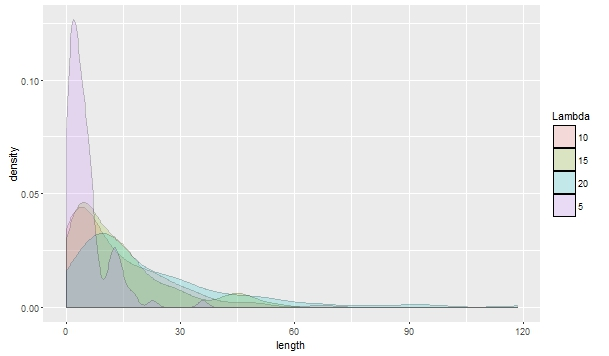
\includegraphics[width=1\linewidth]{Figuras/LAMBDAS}
\caption{Se graficaron distribuciones exponenciales con parámetro $\lambda=5, 10, 15, 20$}
\end{figure}

De aquí nace la siguiente pregunta: dada una observación $ X_0$, ¿cuál sería la $ \lambda_{i}$ que le asigne mayor probabilidad o densidad a la ocurrencia de esta observación? Por ejemplo, de la gráfica anterior se puede observar que si $x_{0}=5$, el mejor valor de lambda sería $\lambda=5$, mientras que si $x_{0}=30$, sería $\lambda=15$. Siguiendo la misma línea de pensamiento, también sería acertado preguntarse por el mejor estimador de $\beta$, donde la probabilidad de que ocurra $\lambda_{i}$ (que maximiza la la probabilidad de ocurrencia de $x_{0}$) sea máxima. Entonces, la función de verosimilitud para $X_{0}$ es:\\
\begin{equation*}
 Lik(\beta|X)=f_{x}(x)=\dfrac{\beta}{(x+\beta)^{2}}=\underset{0}{\overset{\infty }{\int }}f_{x|\lambda}(x)f(\lambda)d\lambda
\end{equation*}

 
Y con el planteamiento anterior, en lugar de buscar el mejor estimador de $\beta$ en Lik($\beta|X_{0}$), podríamos preguntarnos por la mejor $\lambda_{i}$ inducida por $\beta$ tal que $\beta$ maximice la ocurrencia de $\lambda_{i}$, y a su vez, $\lambda_{i}$ maximice la probabilidad de haber observado  $X_{0}$. Entonces con este enfoque, la función de verosimilitud para $X_{0}$ queda expresada de la siguiente manera:

\begin{equation*}
Lik(\lambda_{i},\beta|X_{0})=f_{x|\lambda_{i}}(x|\beta,\lambda_{i})f(\lambda{i})
\end{equation*}
	
	Siguiendo las ideas planteadas previamente, la verosimilitud extendida se define de la siguiente forma:\\
	
	Sean ${X}_{i=1}^{n}$ un conjunto de vectores aleatorios independientes e idénticamente distribuidos de dimensión p con algún vector de parámetros $\theta$, y sea $u$ una variable aleatoria con algún vector de parámetros $\beta$ y con soporte en $R_{+}$, tal que $X_{i}$ se puede esxpresar como una distribución tipo mezcla con variable de mezcla $u$. Entonces  $f_{X_{i}}(x_{i})=\underset{0}{\overset{\infty }{\int }}f_{x_{i}|u}(x_{i})f_{u}(u)du$ para toda $i$, con $X_{i}$ dado $u_{i}$ condicionalmente independiente a $X_{j}$ dado $u_{j}$, y $ u_{i}$ dado $\beta$ independiente a $u_{j}$ dado $\beta$ para toda $i$ diferente de $j$, por lo que la verosimilitud extendida es:\\
	\begin{equation*}
	Lik(u_{i},\theta,\beta |X)=\prod_{i=1}^{n}f_{x_{i}|u_{i}}(x|\theta, u_{i},\beta)f_{u_{i}}(u_{i}|\beta)
	\end{equation*}
	
	
	donde $u_{i}$ es una variable latente.\\
	
	Trabajar con la verosimilitud extendida podría parecer más complicado al tener que estimar una variable latente para cada observación de $X$, pero en ocasiones resulta más sencillo optimizar la función $\prod_{i=1}^{p}f_{x_{i}|u_{i}}(x_{i})f(u_{i})$ que $f(X)$ y, además, existen algoritmos computacionales, vía cadenas de Markov, o el algoritmo EM, que permiten encontrar los estimadores de los parámetros deseados. Por lo qué ahora se hablará brevemente de los distintos y posible métodos a implementar.

%\begin{algorithm}[H]
%	\SetAlgoLined
%	\KwResult{Write here the result }
%	initialization\;
%	\While{While condition}{
%		instructions\;
%		\eIf{condition}{
%			instructions1\;
%			instructions2\;
%		}{
%		instructions3\;
%	}
%}
%\caption{How to write algorithms}
%\end{algorithm}


\subsection{Muestreador de Gibbs}
El muestreador de Gibbs es un método de simulación tipo Markov Chain Montecarlo (MCM), estos métodos permiten obtener muestras de alguna densidad de probabilidad $f_{x}$ mediante la construcción de una cadena de Markov que converga a dicha densidad.\\ 

El muestreador de Gibbs permite obtener una muestra de una distribución conjunta a partir de las distribuciones marginales, por lo que no es necesario conocer la distribución conjunta, basta con construir una cadena de Markov adecuada  con las distribuciones marginales, las cuales convergerán a una muestra aleatoria de la distribución conjunta.\\

De forma intuitiva, el muestreador de Gibbs se plantea de la siguiente manera; supongamos que tenemos una distribución de la forma $f(X,\Theta)$ donde X es un vector aleatorio y $\Theta$ algún vector de parámetors del cual se desearía tener una muestra mediante una cadena de Markov, es decir, obtener una muestra de $f(\theta ^{k}|X)$ a partir de una sucesión de parámetros ${\theta}_{k=1} ^{\infty}$, tal que la probabilidad de transición de esta sucesión converja a la distribución de la cual se desearía tener una muestra, esto es, $\lim_{k->\infty} P(\theta^{k+1}|\theta^{k},X)=P(\theta|X)$. Dada la descripción del modelo anterior, la cadena debe ser estacionaria, irreducible, aperiódica y recurrente positiva. La propiedad de estacionariedad asegurar que $P(\theta|X)$ no cambie cuando $k$ tienda a infinito; irreducible para no descartar ningún valor posible de $\theta ^{k}$ en cada iteración; mientras que, aperiodicidad para que la cadena no tenga ciclos, y así permanecer en el estado estacionario. Por último, recurrente positiva, para que se pueda visitar cualquier estado un número infinito de veces y así asegurar que la distribución límite tomó toda la información disponible en consideración.\\

Ahora bien, para encontrar una cadena que nos permita obtener las caractrísticas anteriores German $\&$ German (citar bien esta parte) demuestra que  $ \lim_{k->\infty} P(\theta^{k}|X)=P(\theta|X)$, donde:
 
 \begin{equation*}
 P(\theta^{k}|X)=\stackrel{~}{{\prod}_{j=1}^{t }}P(\theta_{j}|X,...,\theta_{j-1},\theta_{j+1},...,\theta_{n}) 
 \end{equation*}

 y $\theta_{j}$ dado $X,...,\theta_{j-1},\theta_{j+1},...,\theta_{n}$ es condicionalmente independiente para toda $j$, para alguna medida de probabilidad arbitraria $P(.)$. Entonces si $\theta_{j} ^{k}$ se distribuye $ f(\theta_{j} ^{k}|X,...,\theta_{j-1},\theta_{j+1},...,\theta_{n})$, de aquí se puede obtener facilmente una muestra de $\theta_{j} ^{k}$ para toda $j$, si su densidad tiene una forma cerrada, y así se construiría una cadena de Markov con las caractarísticas deseadas, $[\theta^{k}] _{1} ^{\infty}$, con probabilidad de transición $P(\theta^{k}|X)$.\\

Entonces los pasos para implementar el Muestreador de Gibbs son los siguientes:\\

Dar un conjunto de valores iniciales $\Theta_{0}$, no importa cuáles valores se den, la propiedad de estacionareidad, asegurará la convergencia al estado estacionario. El vector $\theta$ puede ser particionado en d subconjuntos excluyentes, tal que d$<=$n, con la finalidad de simplificar los cálculos. Convenientemente se pueden seleccionar los sobconjuntos de modo que los que tienen alta correlación queden juntos.\\

Para cada $\theta_{j}$ obtener su distribución condicionada \begin{equation*}
f(\theta_{j} |X,...,\theta_{0,j-1},\theta_{0,j+1},...,\theta_{0,n})
\end{equation*} y realizar una simulación de esta. El valor de $\theta_{j}$ obtenido reemplazará a los valores iniciales. En caso de que no se pueda tener la distribución de $\theta|_{X,\theta \ \theta_{j}}$ se realiza un procedimiento de aceptación-rechazo para obtener una realización de $\theta_{j}$.\\

Una vez obtenidos todos los valores de $\theta|_{X,\theta, \ \theta_{j}}$ se reemplazan por los valores iniciales y se repite el procedimiento hasta que la cadena se estabilice.

Computacionalmente el algoritmo se vería de la siguiente forma:\\


%\lstinputlisting[language=R]{h.r}
%\begin{algorithmic}
%	\caption{Muestreador de Gibbs}\label{alg:gibbs}
%	\begin{algorithmic}[1]
%		\Procedure{$\Theta_{k} <- (\theta_{1,0},...,\theta_{d,0})$}{}\Comment{Conjunto de valores iniciales.}
%		\State $r\gets a\bmod b$
%		\For{$r\not=0$}\Comment{We have the answer if r is 0}
%		\State $a\gets b$
%		\State $b\gets r$
%		\State $r\gets a\bmod b$
%		\EndWhile\label{euclidendwhile}
%		\State \textbf{return} $b$\Comment{The gcd is b}
%		\EndProcedure
%	\end{algorithmic}
%\end{algorithmic}


\begin{center}
	$\Theta_{k} <- (\theta_{1,0},...,\theta_{d,0})$\\
	$M<-$ número total de iteraciones.\\
	for $k < M$ \\
		
			$\theta_{j} ^{k+1}<-$ random ($\Pi$($\theta|_{X,\theta^{k} \ \theta_{j} ^{k}}$))\\
		              
	end for\\
\end{center}
									

\section{Algoritmo para la distribución hiperbólica generalizada}

Supongamos que tenemos una colección de $r_{n}$ datos, donde cada $r_{i}\in R^{p}$, de los cuales tenemos motivos para creer que fueron generados por una distribución hiperbólica generalizada p-variada. Entonces nos interesaría inferir los valores de los parámetros de dicha distribución, pero antes de ello sería conveniente expresar a nuestra distribución de interés como una distribución tipo mezcla normal, con variable de mezcla $u$ con distribución Gaussiana inversa (GI), por lo que así podemos replantear el problema, enfocándonos en buscar los parámetros de la distribución de mezcla, $\mu,\beta,\Sigma$.\\

Ahora con un enfoque bayesiano, podemos plantear la verosimilitud de la distribución \textit{aposteriori} de $\mu,\beta,\Sigma$, es decir:
\begin{equation*}
f(\mu,\beta,\Sigma|(r_{i})_{i=1}^{n})=\prod_{i=1}^{n}f_{r_{i}}(r_{i}|\mu,\beta,\Sigma)\Pi(\mu,\beta,\Sigma)
\end{equation*}   
Donde $\Pi(\mu,\beta,\Sigma)$ es la distribución conjunta a \textit{apriori} de $\mu,\beta$ y $\Sigma$, y además asumiremos que tanto $\mu,\beta,\Sigma$ son independientes, por lo que:
\begin{equation*}
f(\mu,\beta,\Sigma|(r_{i})_{i=1}^{n})=\prod_{i=1}^{n}f_{r_{i}}(r_{i}|\mu,\beta,\Sigma)\Pi(\mu|\mu_{0},\Sigma_{0})\Pi(\beta|\mu_{\beta},\Sigma_{\beta})\Pi(\Sigma|S)
\end{equation*}
 Como supuesto adicional, asumiremos que $\mu$ se distribuye $N(\mu_{0},\Sigma_{0})$, $\beta$ se distribuye $N(\beta_{0},\Sigma_{\beta})$, y $\Sigma$ se distribuye $W^{-1}(S,n,p)$. Así, nuestra función de verosimilitud adquiere la siguiente forma:
\begin{equation*}
Lik(\mu,\mu_{0},\beta,\beta_{0},\Sigma,\Sigma_{0},\Sigma_{\beta},S|(r_{i})_{i=1}^{n})=
\end{equation*}
Luego, expresando a nuestra distribución de interés $f_{r_{i}}(r_{i})$ como una distribución tipo mezcla normal, con variable de mezcla $u$, la función de verosimilitud tiene la sigueinte forma:
 
\begin{equation*}
\prod_{i=1}^{n}\int_{0}^{\infty}N_{p}(r_{i}|\mu,u\beta,u\Sigma)GI(u|\lambda_{0},\Psi_{0})g(\mu,\beta,\Sigma)du,
\end{equation*}
donde $g(\mu,\beta,\Sigma)=N_{p}(\mu|\mu_{0},\Sigma_{0})N_{p}(\beta|\beta_{0},\Sigma_{\beta})W_{pxp}(\Sigma|S)$

Por lo que ahora necesitamos conocer también los valores de $\lambda$ y $\Psi$ propios de la distribución gaussiana inversa, para ello supondremos que $\lambda$ y $\psi$ son independientes, y además gracias a la gran flexibilidad de la distribución gamma, asumiremos que cada uno de ellos proviene de una distribución gamma con parámetros $\alpha_{\lambda}$, $\beta_{\lambda}$, $\alpha_{\Psi}$ y $\beta_{\Psi}$, respectivamente, por lo que la distribución \textit{apriori} para $\lambda$ y $\Psi$ está dada de la siguiente manera:

\begin{equation*}
\Pi(\lambda,\Psi)=\Pi(\lambda|\alpha_{\lambda},\beta_{\lambda})\Pi(\Psi|\alpha_{\Psi},\beta_{\Psi})
\end{equation*}

Ahora según lo expuesto en el capítulo 3.algo, es conveniente extender la verosimilitud; esto es que:
\begin{equation*}
Lik(\mu,\beta,\Sigma,(u_{i})_{i=1}^{n},\lambda,\Psi|(r_{i})_{i=1}^{n},\mu_{0},\beta_{0},\Sigma_{\mu},\Sigma_{\beta},S,\alpha_{\lambda},\beta_{\lambda},\alpha_{\Psi},\beta_{\Psi})=
\end{equation*}
\begin{equation*}
\prod_{i=1}^{n}N_{p}(r_{i}|\mu,u_{i}\beta,u_{i}\Sigma)GI(u_{i}|\lambda_{0},\Psi_{0})\Pi(\lambda|\alpha_{\lambda},\beta_{\lambda})\Pi(\Psi|\alpha_{\Psi},\beta_{\Psi}) 
\end{equation*}
\begin{equation*}
N_{p}(\mu|\mu_{0},\Sigma_{0})N_{p}(\beta|\mu_{\beta},\Sigma_{\beta})W^{-1}_{pxp}(\Sigma|S,n,p)
\end{equation*}
Una vez teniendo nuestra función de verosimilitud, ya estamos en condiciones de proponer algún método numérico para encontrar los parámetros de interés; para ello, por un lado se utilizará el muestreador de GIBBS para obtener una muestra de los parámetros buscados; por otro lado se optará por un enfoque bayesiano para tratar la verosimilitud, ya que gracias a este método, podemos aprovechar la información implícita de los datos.\\

Entonces, con un enfoque bayesiano, será necesario encontrar las distribuciones marginales de los parámetros de interés, para que una vez obtenidas se pueda implementar el muestreador de GIBBS.\\ 


Por lo que ahora necesitamos conocer las distribuciones marginales de:
\begin{eqnarray*}
& &\Pi(\mu|\beta,\Sigma,(u_{i})_{i=1}^{n},\lambda,\Psi,(r_{i})_{i=1}^{n},\mu_{0},\beta_{0},\Sigma_{\mu},\Sigma_{\beta},S,\alpha_{\lambda},\beta_{\lambda},\alpha_{\Psi},\beta_{\Psi}) \\
& & \Pi(\beta|\mu,\Sigma,(u_{i})_{i=1}^{n},\lambda,\Psi,(r_{i})_{i=1}^{n},\mu_{0},\beta_{0},\Sigma_{\mu},\Sigma_{\beta},S,\alpha_{\lambda},\beta_{\lambda},\alpha_{\Psi},\beta_{\Psi}) \\
& &\Pi(\Sigma|\mu,\beta,(u_{i})_{i=1}^{n},\lambda,\Psi,(r_{i})_{i=1}^{n},\mu_{0},\beta_{0},\Sigma_{\mu},\Sigma_{\beta},S,\alpha_{\lambda},\beta_{\lambda},\alpha_{\Psi},\beta_{\Psi}) \\
& & \Pi(u_{i}|\mu,\beta,\Sigma,\lambda,\Psi,(r_{i})_{i=1}^{n},\mu_{0},\beta_{0},\Sigma_{\mu},\Sigma_{\beta},S,\alpha_{\lambda},\beta_{\lambda},\alpha_{\Psi},\beta_{\Psi})\\
& & \Pi(\lambda|\mu,\beta,\Sigma,(u_{i})_{i=1}^{n},\Psi,(r_{i})_{i=1}^{n},\mu_{0},\beta_{0},\Sigma_{\mu},\Sigma_{\beta},S,\alpha_{\lambda},\beta_{\lambda},\alpha_{\Psi},\beta_{\Psi}) \\
& &\Pi(\Psi|\mu,\beta,\Sigma,(u_{i})_{i=1}^{n},\lambda,(r_{i})_{i=1}^{n},\mu_{0},\beta_{0},\Sigma_{\mu},\Sigma_{\beta},S,\alpha_{\lambda},\beta_{\lambda},\alpha_{\Psi},\beta_{\Psi})\\
\end{eqnarray*}




%\begin{equation*}
%\Pi(\mu|\beta,\Sigma,(u_{i})_{i=1}^{n},\lambda,\Psi,(r_{i})_{i=1}^{n},\mu_{0},\beta_{0},\Sigma_{\mu},\Sigma_{\beta},S,\alpha_{\lambda},\beta_{\lambda},\alpha_{\Psi},\beta_{\Psi}) 
%\end{equation*}
%\begin{equation*}
%\Pi(\beta|\mu,\Sigma,(u_{i})_{i=1}^{n},\lambda,\Psi,(r_{i})_{i=1}^{n},\mu_{0},\beta_{0},\Sigma_{\mu},\Sigma_{\beta},S,\alpha_{\lambda},\beta_{\lambda},\alpha_{\Psi},\beta_{\Psi}) 
%\end{equation*}
%\begin{equation*}
%\Pi(\Sigma|\mu,\beta,(u_{i})_{i=1}^{n},\lambda,\Psi,(r_{i})_{i=1}^{n},\mu_{0},\beta_{0},\Sigma_{\mu},\Sigma_{\beta},S,\alpha_{\lambda},\beta_{\lambda},\alpha_{\Psi},\beta_{\Psi}) 
%\end{equation*}
%\begin{equation*}
%\Pi(u_{i}|\mu,\beta,\Sigma,\lambda,\Psi,(r_{i})_{i=1}^{n},\mu_{0},\beta_{0},\Sigma_{\mu},\Sigma_{\beta},S,\alpha_{\lambda},\beta_{\lambda},\alpha_{\Psi},\beta_{\Psi})
%\end{equation*}
%\begin{equation*}
%\Pi(\lambda|\mu,\beta,\Sigma,(u_{i})_{i=1}^{n},\Psi,(r_{i})_{i=1}^{n},\mu_{0},\beta_{0},\Sigma_{\mu},\Sigma_{\beta},S,\alpha_{\lambda},\beta_{\lambda},\alpha_{\Psi},\beta_{\Psi}) 
%\end{equation*}
%\begin{equation*}
%\Pi(\Psi|\mu,\beta,\Sigma,(u_{i})_{i=1}^{n},\lambda,(r_{i})_{i=1}^{n},\mu_{0},\beta_{0},\Sigma_{\mu},\Sigma_{\beta},S,\alpha_{\lambda},\beta_{\lambda},\alpha_{\Psi},\beta_{\Psi}) 
%\end{equation*}


\section{Distribuciones marginales completas}

\subsection{Para $\mu$}
Para encontrar la distribución marginal de $\mu|\beta,\Sigma,(u_{i})_{i=1}^{n},(r_{i})_{i=1}^{n}$ a partir de la función de verosimilitud, podemos tomar las densidades donde aparece $\mu$ e identificar su kernel, es decir, de: 

\begin{eqnarray*}
& &\prod_{i=0}^{n}N_{p}(r_{i}|\mu,u_{i}\beta,u_{i}\Sigma)N_{p}(\mu|\mu_{0},\Sigma_{0})=
 \\
& & \prod_{i=1}^{n}\dfrac{exp(-\frac{1}{2}(r_{i}-\mu-u_{i}\beta)'(u_{i}\Sigma)^{-1}(r_{i}-\mu-u_{i}\beta))}{(2u_{i}\Pi)^{p/2}|\Sigma|^{1/2}}\\
& & \dfrac{exp(-\frac{1}{2}(\mu-\mu_{0})'\Sigma_{0}(\mu-\mu_{0}))}{(2\Pi)^{p/2}|\Sigma|^{1/2}}\\
\end{eqnarray*}
%\begin{equation*}
%\prod_{i=0}^{n}N_{p}(r_{i}|\mu,u_{i}\beta,u_{i}%\Sigma)N_{p}(\mu|\mu_{0},\Sigma_{0})=
%\end{equation*}
%\begin{equation*}
%\prod_{i=1}^{n}\dfrac{exp(-\frac{1}{2}(r_{i}-\mu-u_{i}\beta)'(u_{i}\Sigma)^{-1}(r_{i}-\mu-u_{i}\beta))}{(2u_{i}\Pi)^{p/2}|\Sigma|^{1/2}}\dfrac{exp(-\frac{1}{2}(\mu-\mu_{0})'\Sigma_{0}(\mu-\mu_{0}))}{(2\Pi)^{p/2}|\Sigma|^{1/2}}
%\end{equation*}

tomando el cambio de variable  $r_{i}\acute{}=r_{i}-u_{i}\beta$, nos quedamos con:
 \begin{equation*}
 \prod_{i=1}^{n}exp(-\frac{1}{2}(\mu-r_{i}')'(u_{i}\Sigma)^{-1}(\mu-r_{i}'))exp(-\dfrac{1}{2}(\mu-\mu_{0})'\Sigma_{0}(\mu-\mu_{0}))
 \end{equation*}
Después, trabajando únicamente con:
\begin{eqnarray*}
& &\prod_{i=1}^{n}exp(-\frac{1}{2}(\mu-r_{i}')'(u_{i}\Sigma)^{-1}(\mu-r_{i}'))=
 \\
& & exp(-\frac{1}{2}\sum_{i=1}^{n}(\mu-r_{i}')'(u_{i}\Sigma)^{-1}(\mu-r_{i}')) = \\
& &exp(-\frac{1}{2}\sum_{i=1}^{n}(\mu'(u_{i}\Sigma)^{-1}\mu  -2\mu(u_{i}\Sigma)^{-1}r_{i}' -r_{i}'(u_{i}\Sigma)^{-1}r_{i}' )\alpha 
 \\
& &  exp(-\frac{1}{2}\sum_{i=1}^{n}(\mu'(u_{i}\Sigma)^{-1}\mu  -2\mu(u_{i}\Sigma)^{-1}r_{i}')= \\
& & 
exp(-\frac{1}{2}(\mu'(U\Sigma)^{-1}\mu  -2\mu(U\Sigma)^{-1}R), \\
\end{eqnarray*}
donde : 

\begin{equation*}
U=(\sum_{i=1}^{n}\dfrac{1}{u_{i}})^{-1}, R= \sum_{i=1}^{n}\dfrac{r_{i}}{u_{i}}U
\end{equation*}
Entonces, según el anexo 4, a esta parte del kernel de $\mu$ le corresponda una distribución normal p variada con vector de medias $R$, y matriz de varianza covarianza $U\Sigma$. Luego, multiplicando el Kernel anterior por la densidad de $\mu$, y por el anexo 6, se tiene que $\mu$ se distribuye normal con vector de medias:
\begin{equation*}
(R(U\Sigma)^{-1}+\mu_{0}\Sigma_{0}^{-1})(U\Sigma^{-1}+\Sigma_{0}^{-1})^{-1}
\end{equation*}
 y matriz de varianza covarianza:
 \begin{equation*}
 U\Sigma+\Sigma_{0}
 \end{equation*}

\subsection{Para $\beta$}
Mediante un procedimiento similar, encontraremos el Kernel de $\beta$ dado las demás variables de interés. Entonces, de la función de verosimilitud, nos quedamos con la parte donde sólo aparece $\beta$, es decir:
\begin{equation*}
\prod_{i=0}^{n}N_{p}(r_{i}|\mu,u_{i}\beta,u_{i}\Sigma)N_{p}(\beta|\mu_{\beta},\Sigma_{\beta})
\end{equation*}
Luego trabajando con el producto de las n variables normales p variadas correspondientes a $r_{i}$,  considerando los términos que únicamente dependen de $\beta$, y con el cambio de variable $\mu_{i}=r_{i}-\beta$, tenemos que:
\begin{equation*}
\prod_{i=1}^{n}exp(-\dfrac{1}{2}(r_{i}-\mu-u_{i}\beta)'(u_{i}\Sigma)^{-1}(r_{i}-\mu-u_{i}\beta))=
\end{equation*}
\begin{equation*}
exp(-\frac{1}{2}\sum_{i=1}^{n}((u_{i}\beta-\mu_{i})'(u_{i}\Sigma)^{-1}(u_{i}\beta-\mu_{i}))
\end{equation*}

Nuevamente desarrollando el exponente de la función exponencial, y quedándonos únicamente con la parte que depende de $\beta$ tenemos que:
\begin{equation*}
exp(-\dfrac{1}{2}\sum_{i=1}^{n}((u_{i}\beta)'(u_{i}\Sigma)^{-1}(u_{i}\beta)-2(u_{i}\beta)'(u_{i}\Sigma)^{-1}\mu_{i}))=
\end{equation*}
\begin{equation*}
exp(-\dfrac{1}{2}(\beta(V\Sigma)^{-1}\beta-2\beta(V\Sigma)^{-1}VM)
\end{equation*}
Donde:
\begin{equation*}
V=\frac{1}{\sum_{i=1}^{n}u_{i}} , M=\sum_{i=1}^{n}(r_{i}-\mu)
\end{equation*}
 Por lo tanto, según el anexo 4, el Kernel del producto de las n variables normales p-variadas correspondientes a $\beta$ corresponde a una distribución Normal con vector de medias $VM$, y matriz de varianza covarianza $V\Sigma$.
Luego, según el anexo 6, juntando el Kernel obtenido anteriormente con la densidad de $\beta$, se tiene que $\beta$ se distribuye normal p variado con vector de medias: 
\begin{equation*}
(MV\Sigma)^{-1}+\mu_{\beta}'\Sigma_{\beta}^{-1})((V\Sigma)^{-1}+\Sigma_{\beta}^{-1})^{-1}
\end{equation*}
Y matriz de varianza covarianza:
\begin{equation*}
V\Sigma+\Sigma_{\beta}
\end{equation*}

\subsection{Para $\Sigma$}
Para encontrar la distribción marginal de $\Sigma$ a partir de la función de verosmilitud, podemos tomar las densidades donde aparece $\sigma$, y a partir de ahí, identificar el Kernel correspondiente, es decir, tomando: 
\begin{equation*}
\prod_{i=0}^{n}N_{p}(r_{i}|\mu,u_{i}\beta,u_{i}\Sigma)W^{-1}_{pxp}(\Sigma|S,n,p)
\end{equation*}
Y luego trabajando con el producto de las n variables normales p-variadas correspondientes a $r_{i}$, considerando los términos que únicamente dependen de $\Sigma$, y con el cambio de variable $(x_{i}=r_{i}-\mu-\beta)/\sqrt{u_{i}}$, tenemos que:
\begin{eqnarray*}
& &\prod_{i=1}^{n}exp(-\dfrac{1}{2}(r_{i}-\mu-u_{i}\beta)'(u_{i}\Sigma)^{-1}(r_{i}-\mu-u_{i}\beta))\\
& &\dfrac{\exp(-\frac{1}{2}tr(\Sigma^{-1}S))}{|\Sigma|^{n/2}}\\
& =&\dfrac{\exp(-\frac{1}{2}\sum_{i=1}^{n}x_{i}\Sigma^{-1}\sum_{i=1}^{n}x_{i})}{|\Sigma|^{\frac{n}{2}}}\dfrac{\exp(-\frac{1}{2}tr(\Sigma^{-1}S))}{|\Sigma|^{\frac{n}{2}}}
 \\
& =&\dfrac{\exp(-\frac{1}{2}(X\Sigma^{-1}X + tr(\Sigma^{-1}S)))}{|\Sigma|^{n}} \\
& =&\dfrac{\exp(-\frac{1}{2}(tr(\Sigma^{-1}XX') + tr(\Sigma^{-1}S))))}{|\Sigma|^{n}}
 \\
& =&\dfrac{\exp(-\frac{1}{2}(tr(\Sigma^{-1}(XX' + S))))}{|\Sigma|^{n}}
 \\
\end{eqnarray*}

Haciendo $X=\sum_{i=1}^{n}x_{i}$, y ya que $X\Sigma^{-1}X=tr(\Sigma^{-1}(XX')) $. La última expresión corresponde al kernel de una distribución Whishart con matriz de escala $XX'+ S$, y $2n$ grados de libertad.
\section{Para $\lambda$}
Para encontrar la distribción marginal de $\lambda$ a partir de la función de verosmilitud, podemos tomar las densidades donde aparece $\lambda$, y a partir de ahí, identificar el Kernel correspondiente; es decir, de la sigueinte expresión:
\begin{equation*}
\prod_{i=1}^{n}GI(u_{i}|\lambda,\Psi)\Pi(\lambda|\alpha_{\lambda},\beta_{\lambda})
\end{equation*}
nos quedamos con:
\begin{equation*}
\prod_{i=1}^{n}\sqrt{\lambda}\exp(-\frac{\lambda(u_{i}-\Psi)^{2}}{2\Psi^{2}u_{i}}\lambda^{\beta_{\lambda}-1}\exp(-\lambda\alpha_{\lambda})\alpha
\end{equation*}
\begin{equation*}
\lambda^{n/2+\beta_{\lambda} -1}\exp(-X\lambda)
\end{equation*}
donde $X=\sum_{i=1}^{n}\dfrac{(u_{i}-\Psi)^{2}}{2\Psi^{2}u_{i}} - \alpha_{\lambda}$.
Por lo que tenemos que el kernel correponde a una distribución gamma, concluimos que $\lambda$ se distribuye gamma con parámetros $(\frac{n}{2}+\beta_{\lambda}),X$.

\section{Para $\Psi$}
Para encontrar la distribción marginal de $\Psi$ a partir de la función de verosmilitud, podemos tomar las densidades donde aparece $\Psi$, y a partir de ahí identificar el Kernel correspondiente; es decir, de la sigueinte expresión:
\begin{equation*}
	\prod_{i=1}^{n}GI(u_{i}|\lambda,\Psi)\Pi(\Psi|\alpha_{\Psi},\beta_{\Psi})
\end{equation*}
nos quedamos con:
\begin{equation*}
	\prod_{i=1}^{n}\sqrt{\lambda}\exp(-\frac{\lambda(u_{i}-\Psi)^{2}}{2\Psi^{2}u_{i}})\Psi^{\beta_{\Psi}-1}\exp(-\Psi\alpha_{\Psi}) \alpha
\end{equation*}
\begin{equation*}
\exp(-\sum_{i=1}^{n}\frac{\lambda(u_{i}-\Psi)^{2}}{2\Psi^{2}u_{i}})\Psi^{\beta_{\Psi}-1}\exp(-\Psi\alpha_{\Psi}) \alpha
\end{equation*}
\\
El Kernel obtenido resulta difícil de identificar, y tal vez sea complicado obtener la densidad condicional  de $\Psi$, necesaria para implementar el muestreador de GIBBS; por lo que se atacará este problema por medio de una herramienta útil en simulación, llamada slice sampler; la ventaja de utilizar el slice sampler es que nos permite obtener una muestra aleatoria de algúna distribución de probabilidad, con tan solo conocer su Kernel.


\section{Para $u_{i}$}
Para encontrar la distribción marginal de $u_{i}$ a partir de la función de verosmilitud, podemos tomar las densidades donde aparece $u_{i}$, y a partir de ahí identificar el Kernel correspondiente, es decir, de la sigueinte expresión:

\begin{equation*}
\prod_{i=1}^{n}N_{p}(r_{i}|\mu,u_{i}\beta,u_{i}\Sigma)GI(u_{i}|\lambda,\Psi)
\end{equation*}

nos quedamos con:

\begin{eqnarray*}
& &\dfrac{exp(-\frac{1}{2}(r_{i}-\mu-u_{i}\beta)'(u_{i}\Sigma)^{-1}(r_{i}-\mu-u_{i}\beta))}{(u_{i})^{p/2}}\sqrt{\dfrac{1}{u_{i} ^{3}}} \\
& & \exp(-\dfrac{\lambda(u_{i}-\Psi)^{2}}{2\Psi^{2}u_{i}})
 \\
\end{eqnarray*}

EL kernel anterior parece muy difícil de identificar, e intentar encontrar la forma analítica de la distribución condicionada de $u_{i}$ puede resultar muy difícil, si no es que imposible, por lo que optaremos por obtener una muestra aleatoria de $u_{i}$ por medio del slice sampler.\\
Una vez descrita la metodología a emplear para inferir los parámetros de nuesta muestra de interés, ya estamos en condiciones de programar el muestreador de GIBBS y emplearlo para estudiar un conjunto de datos, lo cual se llevará acabo en el siguiente capítulo.

